\documentclass[10pt,landscape]{scrartcl}
\usepackage{multicol}
\usepackage{calc}
\usepackage{ifthen}
\usepackage[landscape]{geometry}
% Umlaute ermöglichen
\usepackage[T1]{fontenc}
% Format dieses Dokuments
\usepackage[utf8]{inputenc}
% Deutsche Trennungsregeln
\usepackage[ngerman]{babel}
\usepackage[babel,german=quotes]{csquotes}
\hyphenation{eine einer eines Entwurf}
\usepackage{listings}
\lstset{emph={%  
    wiederhole, bis, solange, setze, gebe%
    },emphstyle={\bfseries}%
}
%%\usepackage{color}
%\definecolor{lightgrey}{gray}{0.75}
%\definecolor{darkgrey}{gray}{0.25}

\usepackage{amssymb,amsmath}

%% TIKS %%%%%%%%%%%%%%%%%%%%%%%%%%%%%%%%%%%%%%%%%%%%%%%%%
\usepackage{tikz-er2}
\usetikzlibrary{positioning}
\usetikzlibrary{shadows}

\tikzstyle{every entity} = [top color=white, bottom color=blue!30, draw=blue!50!black!100, drop shadow]
\tikzstyle{every weak entity} = [drop shadow={shadow xshift=.7ex, shadow yshift=-.7ex}]
\tikzstyle{every attribute} = [top color=white, bottom color=yellow!20, draw=yellow, node distance=1cm, drop shadow,align=center]
\tikzstyle{every relationship} = [top color=white, bottom color=red!20, draw=red!50!black!100, drop shadow,align=center]
\tikzstyle{every isa} = [top color=white, bottom color=green!20, draw=green!50!black!100, drop shadow]


\usepackage{listings}
\usepackage{color}
\definecolor{lightgrey}{gray}{0.75}
\definecolor{darkgrey}{gray}{0.25}
\lstloadlanguages{SQL} 
\lstset{% general command to set parameter(s)
basicstyle=\footnotesize, 										% print whole listing small
keywordstyle=\color{black}\bfseries, 	% bold black keywords
identifierstyle=, 										% nothing happens
commentstyle=\color{darkgrey},				% grey comments
stringstyle=\ttfamily, 								% typewriter type for strings
showstringspaces=false								% no special string spaces
%numbers=left, 												% show line numbers
%numberstyle=\tiny,										% make line numbers tiny (or small, or large), 
%stepnumber=1, 												% counter for line numbers
%numbersep=5pt												% offset of linenumbers
%backgroundcolor=\color{lightgrey}			% backgroundcolor
}
\lstset{tabsize=4, breaklines=true}
\lstset{
  literate=	{ö}{{\"o}}1
           	{ä}{{\"a}}1
           	{ü}{{\"u}}1
		   	{Ö}{{\"O}}1
		  	{Ä}{{\"A}}1
		   	{Ü}{{\"U}}1
}
\lstset{language=SQL}

\usepackage{ulem}

\usepackage{hyperref}
%\pdfoutput=1
\hypersetup{
	pdfauthor   = {Lazari, Constantin},
	pdftitle    = {Informatik Cheat Sheet (2/4)},
	pdfsubject  = {Informatik},
	pdfkeywords = {},
	pdfcreator  = {Kile},		% Texnic Center oder Kile z.B.
	pdfproducer = {pdflatex},
	colorlinks  = false		% Links nicht farbig hervorheben (sieht Scheisse aus).
} 

% To make this come out properly in landscape mode, do one of the following
% 1.
%  pdflatex latexsheet.tex
%
% 2.
%  latex latexsheet.tex
%  dvips -P pdf  -t landscape latexsheet.dvi
%  ps2pdf latexsheet.ps

% This sets page margins to .5 inch if using letter paper, and to 1cm
% if using A4 paper. (This probably isn't strictly necessary.)
% If using another size paper, use default 1cm margins.
\ifthenelse{\lengthtest { \paperwidth = 11in}}
	{ \geometry{top=.5in,left=.5in,right=.5in,bottom=.5in} }
	{\ifthenelse{ \lengthtest{ \paperwidth = 297mm}}
		{\geometry{top=1cm,left=1cm,right=1cm,bottom=1cm} }
		{\geometry{top=1cm,left=1cm,right=1cm,bottom=1cm} }
	}

% Turn off header and footer
\pagestyle{empty}
 
% Redefine section commands to use less space
\makeatletter
\renewcommand{\section}{\@startsection{section}{1}{0mm}%
                                {-1ex plus -.5ex minus -.2ex}%
                                {0.5ex plus .2ex}%x
                                {\normalfont\large\bfseries}}
\renewcommand{\subsection}{\@startsection{subsection}{2}{0mm}%
                                {-1explus -.5ex minus -.2ex}%
                                {0.5ex plus .2ex}%
                                {\normalfont\normalsize\bfseries}}
\renewcommand{\subsubsection}{\@startsection{subsubsection}{3}{0mm}%
                                {-1ex plus -.5ex minus -.2ex}%
                                {1ex plus .2ex}%
                                {\normalfont\small\bfseries}}
\newcommand{\msout}[1]{\text{\sout{\ensuremath{#1}}}}
\makeatother

% Define BibTeX command
\def\BibTeX{{\rm B\kern-.05em{\sc i\kern-.025em b}\kern-.08em
    T\kern-.1667em\lower.7ex\hbox{E}\kern-.125emX}}

% Don't print section numbers
\setcounter{secnumdepth}{0}
\setlength{\parindent}{0pt}

\setlength{\parskip}{0pt plus 0.5ex}

\def\ojoin{\setbox0=\hbox{$\bowtie$}%
  \rule[-.02ex]{.25em}{.4pt}\llap{\rule[\ht0]{.25em}{.4pt}}}
\def\leftouterjoin{\mathbin{\ojoin\mkern-5.8mu\bowtie}}
\def\rightouterjoin{\mathbin{\bowtie\mkern-5.8mu\ojoin}}
\def\fullouterjoin{\mathbin{\ojoin\mkern-5.8mu\bowtie\mkern-5.8mu\ojoin}}

% -----------------------------------------------------------------------

\begin{document}

	\raggedright
	\footnotesize
	\begin{multicols}{3}


	% multicol parameters
	% These lengths are set only within the two main columns
	%\setlength{\columnseprule}{0.25pt}
	\setlength{\premulticols}{1pt}
	\setlength{\postmulticols}{1pt}
	\setlength{\multicolsep}{1pt}
	\setlength{\columnsep}{2pt}
	\newlength{\MyLenA}
	\newlength{\MyLenB}

	\begin{center}
	\Large{\textbf{Datenbanken Cheat Sheet}} \\
	\end{center}

	\section{Begriffe}
\begin{description}
 \item [Information] (lat. \enquote{informatio}, Form oder Gestalt geben) ist nicht einheitlich
 definiert. Im allgemeinen wird darunter \enquote{übertragenes Wissen} verstanden.
 \item [Daten] (lat. \enquote{datum}, gegebenes) ebenfalls nicht einheitlich definiert. Grundsätzlich
 codierbare Angaben über Dinge oder Sachverhalte, die gespeichert und verarbeitet werden können.
 Die jährlich produzierte Datenmenge liegt bei ca. 10 Zettabytes ($10^{21}$ Bytes)
 \item [strukturierte Daten] haben eine explizite Struktur und sind in der Minderheit (Bsp. Tabellen)
 \item [unstruktierte Daten] haben keine explizite Struktur (ggf. implizite Struktur aufgrund einer
 zugrunde liegenden Grammatik. (Bsp. Text, Bilder, Filme, \dots)
 \item [semistrukturierte Daten] sind nur zum Teil strukturiert (Bsp. XML)
\end{description}

\subsection{Dateisystem vs. DBMS}
\subsubsection{Dateisystem}
Daten werden in Dateien vom Betriebssystem verwaltet. Anwendungen lesen/schreiben die Daten direkt. (Office-Anwendungen,
Buchhaltungssoftware, \dots)


% \begin{tabular}{
% 	@{}p{\linewidth/2}|
% 	@{}p{\linewidth/2}}
% 	\multicolumn{1}{c}{Vorteile} & \multicolumn{1}{c}{Nachteile}\\
% 	\begin{minipage}{\linewidth}
		\begin{itemize}
			\item [$+$] einfach, angepasst, effizient
			\item [$+$] keine Rücksicht auf andere
			\item [$+$] proprietäre Formate möglich
% 		\end{itemize}
% 	\end{minipage}
% 	&
% 	\begin{minipage}{\linewidth}
% 		\begin{itemize}
			\item [$-$] Verwendung für unterschiedliche Zwecke problematisch
			\item [$-$] i.d.R. Strukturänderung $\Rightarrow$ Programmänderung 
			\item [$-$] Synchroner Zugriff aufwändig zu realisieren
			\item [$-$] Abgestufte Zugriffsrechte aufwänding zu realisieren
			\item [$-$] Daten häufig mehrfach gespeichert
			\item [$-$] Datenaustausch, -integration komplex
		\end{itemize}
% 	\end{minipage}	
% \end{tabular}

\subsubsection{Datenbanksysteme}
Verwalten und nutzen (sehr) grosse Datenmengen. Der Zugriff ist deklarativ und mengenorientiert.
Die Daten werden einmalig und zentral definiert. Wichtige Aufgaben (Integritätskontrolle, Redundanzverwaltung,
Zugriffskontrolle und -optimierung, synchroner Zugriff, zentrale Datensicherung und Wiederherstellung) 
können so automatisiert werden. Allerdings sind Aufbau und Betrieb eines Datenbanksystems anspruchsvoll und teuer.


\subsection{Datenunabhängigkeit (DU)}
\begin{description}
	\item [Logische DU] Anwendungsprogramme müssen die logische Gesamtstruktur nicht kennen,
	um spezifische Verarbeitungen vorzunehmen $\Rightarrow$ sie sind von Datenbankschema-Änderungen
	nicht betroffen.
	\item [Physische DU] Anwendungsprogramme müssen die interne Organisation der Daten und Zugriffs- 
	und Speicherungsmöglichkeiten nicht kennen $\Rightarrow$ sie sind von Speicher- und Zugriffstrukturänderungen
	nicht betroffen
\end{description}

\subsection{Datenbank Management Systeme}
\textbf{DB-Typen:} hierarchisch, relational, objekt-relational, objektorientiert, deduktiv, netzwerk, \dots

Ein Datenbanksystem (DBS) besteht aus einem Datenbankverwaltungssystem (Software, DBMS) und einer Datenbank (Daten, DB).
Anwendungsprogramme kommunizieren mit dem DBMS. Anwendungsprogramme und DBS bilden ein Informationssystem (IS).

\subsubsection{Aufgaben DBMS}
Syntaxprüfung, Objekte und Zugriffsrechte prüfen, Metadaten lesen, Zugriffsmodul generieren, Transaktionskontrolle,
Daten lesen, Daten zusammenstellen, Daten ausgeben.

% \begin{tabular}{@{}p{\linewidth/2}|@{}p{\linewidth/2}}
%  \multicolumn{1}{c}{Dateisystem} & \multicolumn{1}{c}{Datenbank} \\\hline
%  + einfach, anpassbar, effizient & + langfristige Aufbewahrung\\
%  + Proprietäre Formate möglich & + grosse Mengen\\
%  + Keine Rücksicht auf ander & + viele Benutzer\\
%  - Struktur = Programmänderung & + einfache Rechteverwaltung\\
%  - Simultaner Zugriff schwierig & + logische Unabhängigkeit\\
%  - abgest. Zugriffsrechte schwierig & + physische Unabhängigkeit\\
%  - Mehrfachverwendung heikel &  + Automatisierung\\
%  - Logische \& physische abhängig & - teuer und aufwändig\\
% \end{tabular}

\subsubsection{ANSI-SPARC-3-Ebenen-Architektur (1975)}
\begin{description}
 \item [Extern] Sicht einzelner Anwendungen oder Benutzergruppen
 \item [Konzeptionell] Logische Gesamtsicht
 \item [Intern] Speicherung, Datenorganisation, Zugriffsstrukturen
\end{description}

\subsubsection{Aufbau und Betrieb}
Auf- und Ausbau bezeichnet das (iterative) erstellen verschiedener Datenbank Schemas, 
häufig im laufenden Betrieb. Betrieb, Nutzung und Verwaltung (Anzeigen, Einfügen, Ändern, Löschen, Backup, Restore)
mit Hilfe der Daten-Manipulationssprache (DML)
	
	\section{Relationenmodell (E. F. Codd (1970))}

\begin{description}
	\item [Domäne] Auch Wertebereich oder Datentyp: definiert die zulässigen Werte (Ganze Zahlen, Zeichenketten, \dots)
	als Mengen und sind nicht weiter strukturiert.
	\item [Attribut] besteht aus zwei Teilen: einem Namen und einer Domäne. Attribute können den Wert \texttt{NULL} haben.
	\item [Tupel] bezeichnet ein atomares Datenelement aus gewerteten zusammengehörenden Attributen
	\item [Relation] besteht aus zwei Teilen:
	\begin{enumerate}
		\item Schema, Heading, Intension: Name, Namen und Typen der Attribute
		\item Instanz, Extension: Zeilen (n-Tupel von Werten)
	\end{enumerate}
	Grundsätzlich ist eine Relation $R$ eine Teilmenge des kartesischen Produkts verschiedener Mengen (hier der Wertebereiche).
	$R \subseteq W_1, \times W_2 \dots \times W_n$. Dargestellt als $R(A_1, A_2, \dots, A_n)$ ($A_i$ steht für Attribut $i$).
	Relationen sind äquivalent ($R_1 \sim R_2$) wenn sie die gleichen Attribute enthalten. Relationen sind dublikatfrei, ungeordnet, 
	endlich und in der ersten Normalform (alle Attribute haben atomare Typen). Als Tabelle: Spalten entsprechen Attributen, die Anzahl der Spalten entspricht dem Grad,
	die Zeilen entsprechen Tupeln und der Anzahl der Zeilen entspricht der Kardinalität.
	\item [Beziehung] Eine Beziehung zwischen Relationen werden über Attribute und ihre Werte hergestellt.
	\item [Schlüssel] identifizieren eindeutig Tupel einer Relation. Sie sind ein Attribut oder eine Attributskombination,
	die jedes Tupel eindeutig identifiziert und deren Wert sich während der Existenz des Tupels nicht ändert.
\end{description}



	
	\section{Relationale Algebra}
Vereinigungskompatibel:
\begin{enumerate}
	\item Gleiche Anzahl Attribute (gleiche Namen nicht notwendig)
	\item Übereinstimmende Attribute haben den gleichen Typ (Domäne).
\end{enumerate}

\subsection{Vereinigung ($R_1 \cup R_2$)}
ergibt die Menge aller Tupel, die in $R_1$ oder $R_2$ vorkommen (ohne doppelte). Voraussetzung: $R_1$ und $R_2$ sind vereinigungskompatibel.
Es gilt das Kommuntativ-Gesetz: $R_1 \cup R_2 = R_2 \cup R1$

\subsection{Durchschnitt ($R_1 \cap R_2$)}
ergibt die Menge aller Tupel, die in $R_1$ und $R_2$ vorkommen (ohne doppelte). Voraussetzung: $R_1$ und $R_2$ sind vereinigungskompatibel.
Es gilt das Kommuntativ-Gesetz: $R_1 \cap R_2 = R_2 \cap R1$

\subsection{Differenz ($R_1 - R_2$ bzw. $R_1 \setminus R_2$)}
ergibt die Menge aller Tupel, die in $R_1$ und nicht in $R_2$ vorkommen. Voraussetzung: $R_1$ und $R_2$ sind vereinigungskompatibel.
Das Kommuntativ-Gesetz gilt nicht.

\subsection{Produkt ($R_1 \times R_2$)}
ergibt die Menge aller Tupelkombinationen beider Relationen (ohne doppelte).
Das Kommuntativ-Gesetz gilt nicht, aber $R_1 \times R_2 \sim R_2 \times R_1$.
(Es gäbe auch noch die praktisch bedeutungslose Division).

\subsection{Selektion ($\sigma_P (R)$)}
$P$ steht das Prädikat, die Selektionsbedingung. Die Selektion ergibt die Menge aller Tupel aus $R$ für die $P$ gilt.
Die Selektion hat nichts mit der Reihenfolge (Sortierung) zu tun.

\subsection{Projektion ($\pi_L (R)$)}
$L$ steht für die Attributkombination aus $R$. Die Projekt ergibt die Menger aller Attribute aus $R$, die $L$ sind.
Theoretisch werden doppelte eliminiert.

\subsection{Verbund, Join ($R_1 \Join R_2$)}
ergibt die Verkettung der Attribute von $R_1$ mit den von $R_2$ bei denen gemeinsame, vereinigungskompatible Attribute gleich sind.
Verknüpfbar sind zwei Tupel, wenn sie in allen gemeinsamen Attributen übereinstimmen.
\settowidth{\MyLenA}{Right outer join ($L \fullouterjoin R$)~~}
\begin{tabular}{
	@{}p{\the\MyLenA}%
	@{}p{\linewidth-\the\MyLenA}}
	Natural, Auto Join & $\sigma_{R_1.s_1 = R_2.s_1 \wedge R_1.s_2 = R_2.s_2 \dots}$\\
	Equi-Join & Prüfung nur auf Gleichheit. Attribute mit logischem Und verknüpft.\\
	Theta Join ($L \Join _\theta R $) & Kartesisches Produkt mit Selektion (bsp. $R_1.a_1 > R_2.a_2$)\\
	Cross Join & keine gemeinsamen Attribute (kartesisches Produkt)\\
	Semi Join ($L \ltimes R$) & Natural Join, nur Attribute von $L$\\
	Left outer join ($L \leftouterjoin R$) & Alle von Tupel von $L$ mit \texttt{NULL} für Attribute von $R$, die nicht verknüpfbar sind.\\
	Right outer join ($L \rightouterjoin R$) & Alle von Tupel von $R$ mit \texttt{NULL} für Attribute von $L$, die nicht verknüpfbar sind.\\
	Full outer join ($L \fullouterjoin R$) & Alle von Tupel von $L$ und $R$ mit \texttt{NULL} für Attribute, die nicht verknüpfbar sind.\\  
\end{tabular}





	
	\section{Funktionale Abhängigkeit}
Das Attribut bzw. die Attributskombination $Y$ ist funktional abhängig vom
Attribut bzw. von der Attributskombination $X$ derselben Relation $R$, wenn
zu einem bestimmten Wert von $X$ höchstens ein Wert von $Y$ möglich ist ($X \rightarrow Y$)

\subsection{Regeln}
\settowidth{\MyLenA}{Pseudotransitivität~~}
\begin{tabular}{
	@{}p{\the\MyLenA}%
	@{}p{\linewidth-\the\MyLenA}}
	Projektivität & $(\{Y\} \subseteq \{X\}) \Rightarrow (X \rightarrow Y)$\\
	Distributivität & $(X \rightarrow YZ) \Rightarrow (X \rightarrow Y, X \rightarrow Z)$\\
	Additivität & $(X \rightarrow Y, X \rightarrow Z) \Rightarrow (X \rightarrow YZ)$\\
	Transitivität & $(X \rightarrow Y, Y \rightarrow Z) \Rightarrow (X \rightarrow Z)$\\
	Pseudotransitivität & $(X \rightarrow Y, YW \rightarrow Z) \Rightarrow (XW \rightarrow Z)$\\
	Akkumulation & $(X \rightarrow YZ, Z \rightarrow W) \Rightarrow (X \rightarrow YZW)$\\
	Erweiterung & $(X \rightarrow Y, W \rightarrow Z) \Rightarrow (XW \rightarrow YZ)$\\
\end{tabular}

	
	\section{Datenbank-Entwicklung}
\settowidth{\MyLenA}{Anforderungsanalyse~~}
\begin{tabular}{
	@{}p{\the\MyLenA}%
	@{}p{\linewidth-\the\MyLenA}}
	Anforderungsanalyse, Spezifikation & Datenanforderungen durch Interviews, Fragebögen ermitteln\\
	Konzeptioneller Entwurf & Konzeptionelles Model beschreiben (DBMS unabhängig) $\Rightarrow$ Konzeptionelles Schema\\
	Logischer Entwurf & Logisches Schema aus dem Datenmodell erstellen, optimieren, externe Schemas definieren (DBMS abhängig) $\Rightarrow$ Logisches Schema\\ 
	Physischer Entwurf & Internes Schema definieren (DBMS abhängig) $\Rightarrow$ Physisches Schema\\
	Deklaration Schemas & In der DDL des DBS\\
\end{tabular}

Kriterien: Vollständigkeit, Korrektheit, minimale Redundanzen, Lesbarkeit, Erweiterbarkeit, Normalisierung.

Refactoring eines Modelles ist sehr aufwändig und wird deswegen kaum gemacht. Daher am besten mit einem kleinen
Kernteam (Business Spezialist (Anforderungen/Konzept), Datenmodellierer(Konzept/Logik), Datenbank Designer(Logik/Physisches Model)) arbeiten, das Entwürfe macht, die von einem grösseren Team
(Datenbankspezialisten, Projektmanager, Auftraggeber) evaluiert werden.

\begin{description}
	\item [Konzeptionelles Modell] weitgehend technologie-unabhängige Spezifikation der Daten, die in der Datenbank
		gespeichert werden sollen
	\item [Logisches Modell] Übersetzung des konzeptionellen Schemas in Strukturen, 
		die mit einem konkreten DBMS implementiert werden können
	\item [Physisches Modell] alle Anpassungen, die nötig sind um eine befriedigende Leistung im Betrieb zu erreichen
		(Datenverteilung,  Indexierung,  ...)
\end{description}


	
	\section{Datenmodellierung}
Daten- und funktionale Anforderungen definieren. Anschliessend auf die Daten Abstraktionskonzepte anwenden:
Klassifikation (gleiche oder ähnliche \enquote{Dinge}), Aggregation (Zusammenfassen von \enquote{Dingen}, Name, Strasse, \dots zu Adresse),
Generalisierung und Spezialisierung (Verallgemeinerung, Teilmengenbeziehungen, Zerlegung in disjunkte Untermengen).

Bei der Modellierung gilt es sich auf den Anwendungsbereich zu beschränken. Die Modellierung muss unabhängig von der 
späteren Implementierung sein.

\subsection{Entity-Relationship-Model (P. P. S. Chen, 1976)}
\begin{description}
	\item [Entität] Ein  konkretes  oder  abstraktes  Objekt  der  realen  oder  einer  
Vorstellungswelt, welches eindeutig identifiziert werden kann. Eine Entität hat Attribute (Bsp. Herr Aebi). 
	\item [Entitätsmenge] Gleichartige Entitäten, d.h. Entitäten mit denselben Eigenschaften (Bsp. Personen).
	\item [Identifikationsschlüssel] Ein Attribut oder eine Menge von Attributen, welche eine Entität eines
Entitätstyps innerhalb dieses Typs eindeutig identifiziert (Bsp. Personalnummer)
	\item [Beziehung] Eine Beziehung zwischen Entitäten $e_1, e_2, \dots, e_n (n \geq 2)$ ist ein $n$-
Tupel, wobei jedes $e_i$ eine Entität eines Entitätstyps $E_i (1 \leq i \leq n)$ ist. Wenn derselbe Entitätstyp mehrfach 
vorkommt ($E_i$ und $E_j$ mit $i \neq j$), dann müssen deren verschiedene Rollen mit Hilfe zusätzlicher
Rollennamen bezeichnet werden.\\
	Gleichartige Beziehungen werden zu einem Beziehungstyp zusammengefasst (Bsp. Person als Autor eines Buches)
	Identifikationsattribute einer Entität, die an einer Beziehung beteiligt ist, gehört implizit zur Beziehung.
	Eine Beziehung kann darüber hinaus weitere Attribute haben. Der Identifikationschlüssel einer Beziehung wird
	aus Identifikationsattributen, der an der Beziehung beteiligten Entitätstypen gebildet.
	\item[Generalisierung (is-a)] Eine Generalisierung ist ein Enitätstyp $G$ der die gemeinsamen Attribute der
	spezialisierten Entitäten $E_1, E_2, \dots, E_n$ umfasst.
	Eine Spezialisierung ist disjunkt, wenn $\bigcap (E_1, E_2, \dots, E_n) = \emptyset$. Ansonsten ist er überdeckend.
\end{description}

\begin{center}
\scalebox{.87}{
\begin{tikzpicture}[node distance=1cm, every edge/.style={link}]
	\node[entity] (entity) {Entität};
	\node[attribute] (key) [above left=of entity] {\key{Schlüssel}} edge (entity);
	\node[attribute] (attribute) [left=of entity] {Attribut} edge (entity);
	\node[multi attribute] (mattribute) [below left=of entity] {Multiattribut} edge (entity);
	\node[relationship] (rel) [right=of entity] {Beziehung} edge (entity);
	\node[attribute] (relAttr) [below=of rel] {Bez.-Attribut} edge (rel);
	\node[isa] (isa) [below=of entity] {ISA} edge (entity);
\end{tikzpicture}
}
\end{center}

\subsection{Beziehungstypen (Kardinalität)}
\begin{description}
	\item [1:1] Jedem Element aus $E_1$ ist höchstens 1 Element aus $E_2$ zugeordnet
	\item [1:M] Jedem Element aus $E_1$ können beliebig viele Elementa aus $E_2$ zugeordnet sein,
	jedem Element aus $E_2$ aber höchstens ein Element aus $E_1$
	\item [M:M] Jedem Element aus $E_1$ können beliebig viele Elemente aus $E_2$ zugeordnet sein
	und umgekehrt. Diese Beziehungen müssen für Datenbanken aufgelöst werden.
\end{description}

Attribute werden aus Gründen der Übersichtlichkeit im ERM oft weggelassen und in ergänzenden Dokumenten festgehalten.
Die Details entstehen in der Regel beim logischen Entwurf. Der Entwurf ist ein iterativer Prozess an dem mehrere
Personen beteiligt sein sollten.  

\section{Logischer Entwurf}
Grundsätzlich wird aus einer Entität eine Relation, ebenso wird aus einer Beziehung eine Relation. Mehrwertige Attribute
werden aufgeteilt (zusätzliche Relationen), M:M Beziehungen werden mit Zwischentabellen aufgelöst (zusätzliche Relationen).

Am Ende steht ein logisches Schema, das in SQL (DDL) formuliert ist.

\subsection{Normalisierung}
Unsachgemässe Entwürfen können zu Mutationsanomalien (unerwünschte Auswirkung von Änderungen) führen. Durch
Normalisierung wird dies verhindert.

Anwendungswissen für die Normalisierung: Repetitionsgruppen (was kommt wie oft vor?), Schlüssel, funktionale Abhängigkeiten,
Codierungen.

\begin{description}
	\item [1. Normalform] Alle Attribute enthalten nur atomare Werte (mehrwertige Attribute werden in Tupel umgewandelt)
	\item [2. Normalform] Eine Relation ist in der zweiten Normalform, wenn die erste Normalform vorliegt 
	und jedes Nichtschlüsselattribut vom Primärschlüssel voll funktional abhängig ist. (Mehrere Tabellen entstehen)
	\item [3. Normalform] Die dritte Normalform ist erreicht, wenn sich das Relationenschema in 2NF befindet, und jedes 
	Nichtschlüsselattribut von keinem Schlüsselattribut transitiv abhängt.
\end{description}

\subsubsection{1NF $\rightarrow$ 2NF}
\begin{enumerate}
	\item Bestimme alle Nichtschlüsselmerkmale, die bereits von einem Teilschlüssel funktional abhängig sind.
	\item Bilde aus den Teilschlüsseln und allen von ihnen funktional abhängigen Nichtschlüsselmerkmalen eigene Tabellen.
	\item Entferne aus der ursprünglichen Tabelle alle nicht voll funktional abhängigen Nichtschlüsselmerkmale.
\end{enumerate}

\subsubsection{2NF $\rightarrow$ 3NF}
\begin{enumerate}
	\item Bestimme alle vom Schlüssel transitiv abhängigen Nichtschlüsselmerkmale.
	\item Bilde aus diesen transitiv abhängigen Nichtschlüsselmerkmalen und den Nichtschlüsselmerkmalen, 
	von denen sie funktional abhängig sind, eigene Tabellen.
	\item Entferne aus der ursprünglichen Tabelle alle transitiv abhängigen Nichtschlüsselmerkmale.
\end{enumerate}

Durch Normalisierung werden Redundanzen vermindert und Anomalien vermieden. Allerdings entstehen so 
viele kleine Relationen, die einen hohen Verarbeitungsaufwand nach sich ziehen (Update-Query-Tradeoff).
	
	\section{Physischer Entwurf}
Der Vorgang ist iterativ. Tuning erfolgt während des laufenden Betriebs.

\begin{itemize}\itemsep0em
	\item Speichermedium wählen (RAID 0, 1, 5)
	\item Zugriffsart
	\item Block-, Seitenzuweisung, Verteilung der Daten
	\item Indexierung
	\item Monitoring
	\item Denormalisierung
\end{itemize}

\subsection{Speicherhierarchie}
Je schneller, desto kleiner, desto teurer ...
\begin{enumerate}\itemsep0em
	\item Cache Speicher
	\item Arbeits-, Programmspeicher
	\item Massenspeicher, Festplatte, USB-Stick
	\item Archiv-Speicher (Magnetbänder, optische Platten)
\end{enumerate}

\subsubsection{Festplatten}
%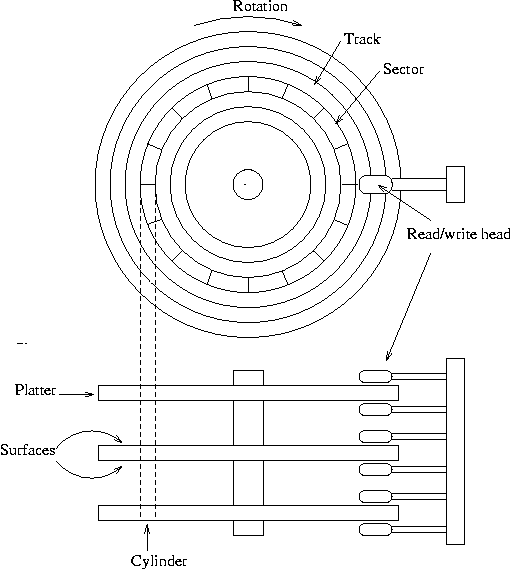
\includegraphics[width=\linewidth]{hd-schematic.png}
bestehen aus einem Plattenstapel. Eine Platte ist in Spuren (Tracks), diese in Sektoren unterteilt. 
Übereinanderliegende Spuren heissen Zylinder. Mehrere Spuren bilden einen Block.

Daten werden blockweise geschrieben/gelesen. Es werden immer ganze Blöcke übertragen.

Das DBMS stellt einen Disk Space Manager (verwaltet Zugriff auf Sekundärspeicher) und einen Buffer Manager
(verwaltet den Hauptspeicher) zur Verfügung. Das Betriebssystem gewährt mit dem Platten-Controller den Zugriff.

\subsection{Datenorganisation}
\settowidth{\MyLenA}{Unsortierte Daten~~}
\begin{tabular}{
	@{}p{\the\MyLenA}%
	@{}p{\linewidth-\the\MyLenA}}
	Unsortierte Daten & Sequentielle Suche ($\frac{n}{2}$ Zugriffe)\\
	Sortierte Daten & Binäre Suche ($\log_2 n$ Zugriffe)\\
\end{tabular}\\
$n =$ Anzahl Datensätze. Sortierung nur für ein Kriterium möglich. Indexe sind verschiedene sortierte Verzeichnisse.
Aber: Indexe brauchen zusätzlichen Speicherplatz und müssen gepflegt werden (Update-Query-Tradeoff)
Indexe sind das primäre Optimierungsmittel!

\begin{itemize}\itemsep0em
	\item [$+$] Primärschlüssel (i.\,d.\,R. automatisch)
	\item [$+$] Fremdschlüssel (beschleunigt Joins)
	\item [$+$] Attribute mit häufigen Abfragen und kleinen Resultatmengen
	\item [$+$] Attribute, die oft sortiert ausgegeben werden
	\item [$-$] Attribute, deren Wert sich häufig ändert
	\item [$-$] Grosse Attribute, komplexe Attributkombinationen
\end{itemize}

\subsubsection{Datenorganisationsformen}
\begin{description}
	\item [Heap-Datei] Bei einer Heap-Datei werden die Datensätze unsortiert hintereinander (sequentiell) geschrieben.
	Einfach, aber nur sequentielle Suche ist möglich (Suchen, bis gefunden).
	\item [Hash-Verfahren] Dabei werden die Datensätze unterschiedlichen Bereichen zugeordnet. Innerhalb der Bereiche 
	sind die Datensätze wieder ungeordnet. Die Zuordnung der Datensätze zu den Bereichen erfolgt über eine Hashfunktion.
	Einfach, aber einzelne Bereiche müssen sequentiell durchsucht werden.
	\item [ISAM-Verfahren] Beim ISAM-Verfahren (Index Sequential Access Method) wird neben der eigentlichen Datendatei, 
	die die Datensätze in sortierter Reihenfolge enthält, eine weitere Datei, die so genannte Index-Datei gepflegt. 
	Diese Index-Datei ermöglicht einen beschleunigten Zugriff auf die Daten. Suchen ist sehr schnell, aber die Index-Datei
	muss ständig mit angepasst werden.
	\item [B$^*$-Baum-Verfahren] Betrachtet man die Indexdateien des ISAM-Verfahrens wiederum als Datensätze, so kann zu diesen Datensätzen wiederum eine Indexdatei
	generiert werden. Durch diese Verschachtelung von Indexdateien kommt man zu einer baumartigen Struktur. 
	Merkmale eines B*-Baumes:
	\begin{itemize}\itemsep0em
		\item Jeder Knoten des Baumes kann mehrere Kindknoten haben (Mehrwegbaum)
		\item Der Baum ist ausgeglichen (balancierter Baum)
		\item Die Knoten enthalten nur Verweise und nicht die eigentlichen Daten
	\end{itemize}
	Es gibt so zwar keine grossen Index-Dateien, doch einfügen und löschen ist kompliziert. Die optimale Variante
	für überwiegend lesenden Zugriff.
	\item [Sekundärindex] Index über ein zusätzliches Merkmal. Lesender Zugriff auf zusätzliches Merkmal ist sehr schnell, aber einfügen und
löschen ist noch komplizierter als beim B$^*$-Baum-Verfahren.
\end{description}

\subsection{Anfrageoptimierung}
Die Anzahl Diskzugriffe sind zu minimieren. Dabei werden Abfragebäume visualisiert und mit Hilfe der relationalen Algebra
optimiert (Kommutativität, Relationen mit höherer Kardinalität in die innere Schleife (Nested-Loop-Join), sortieren vor
dem mischen (Sort-Merge-Join), mit Selektion und Projektion Zwischenergebnisse verkleinern.

Die Optimierung hängt oft vom konkreten Datenvolumen ab.

\subsubsection{Regeln}
\begin{itemize}
	\item Verbund ($\Join$), Vereinigung ($\cup$), Durchschnitt ($\cap$) und Produkt ($\times$) 
	sind kommutativ und assoziativ. 
	\item Selektionen sind vertauschbar: $\sigma_P(\sigma_Q(R)) = \sigma_Q(\sigma_P(R))$
	\item Konjunktionen in einer Selektionsbedingung kann in mehrere Selektionen aufgebrochen werden:
	$\sigma_{P_1}(R) \wedge \sigma_{P_2}(R) \wedge \dots \wedge \sigma_{P_n}(R) = \sigma_{P_1}(\sigma_{P_2}(\dots(\sigma_{P_n}(R))))$
	\item Projektion mit Vereinigung vertauschbar: $\pi_L(A \cup B) = \pi_L(A) \cup \pi_L(B)$
	\item Disjunktion in Konjunktion umwandelbar: $\neg (A \wedge B) = \neg A \vee \neg B, \neg (A \vee B) = \neg A \wedge \neg B$
\end{itemize}
Das DBMS nutzt diese Regeln.
\begin{itemize}\itemsep0em
	\item Wenn möglich vor dem Join sortieren
	\item Wenn Nested-Loop-Join notwendig, vor dem Join einschränken ($\sigma, \pi$)
	\item Indexe reduzieren den Aufwand, kosten aber Aufwand ($n \log_n)$).
\end{itemize}

\subsubsection{Optimierter Abfragebaum}
	\begin{tikzpicture}[
		leaf/.style={rectangle, draw=black, fill=black!10, text width=3cm, drop shadow, text centered},
		node/.style={text width=1cm, text centered},
		line/.style={thick, shorten >=2pt},
		node distance=0.5cm
		]
	\node [node] (projection) {\Large{$\pi$} \normalsize Titel};
 	\node [anchor=west, text width=1cm, left=0.5cm of projection] (note0) {Mng: 1};
 	\node [node, below=of projection] (select) {\Large{$\sigma$}};
	\node [anchor=west, text width=1cm, left=0.5cm of select] (note1a) {Mng: 2};
 	\node [anchor=west,text width=2cm, right=0.5cm of select] (note1b) {\small Ta.Aa = Tb.Ab};
 	\draw [line] (projection) -- (select);

 	\node [node, below=of select] (join) {\Large{$\Join$}};
 	\node [anchor=west, text width=2cm, left=0.5cm of join] (note2) {Mng: 3};
 	\draw [line] (select) -- (join);
	\node [below left=0.25cm of join, text width=4cm, text centered] (sigmaBook) {\Large{$\sigma$} \small Fachgebiet\\= \enquote{Theor. Inf.}\\\normalsize{Menge: 3}};
	\node [below right=0.25cm of join, text width=4cm, text centered] (sigmaLector) {\Large{$\sigma$} \small PersNr\\= \enquote{866778}\\\normalsize{Menge: 1}};
 	\node [leaf, below=of sigmaBook] (book) {Buch};
 	\node [anchor=west, text width=2cm, text centered, below=0.5cm of book] (note3) {Mng: 19};
 	\node [leaf, below=of sigmaLector] (lector) {Lektor};
 	\node [anchor=west, text width=2cm, text centered, below=0.5cm of lector] (note4) {Mng: 6};
 	\draw [line] (join) -- (sigmaBook);
 	\draw [line] (join) -- (sigmaLector);
	\draw [line] (book) -- (sigmaBook);
	\draw [line] (lector) -- (sigmaLector);
	\end{tikzpicture}\\
%

\textbf{Anfragebeispiel:}	$\pi_{t1.f1, t2.f1} (\sigma_{t1.f1 = \mbox{\enquote{kriterium}}}(t1 \Join t2))$


	
	\section{SQL (IBM 1974)}
Zwar gibt es einen Standard, doch eingesetzte Systeme sind proprietär. Einerseits aus kommerziellen, andererseits aus
Trägheitsgründen - das SQL-Komitee hingt den Bedürfnissen des Marktes hinterher.

Leider ist SQL für \enquote{reale} Anwendungen zu wenig mächtig. (Keine Benutzerschnittstellen, komplexe Berechnungen nicht möglich,
Zugriff auf Geräte nicht möglich, Vernetzung problematisch) $\Rightarrow$ SQL wird mit Programmiersprachen (Java/JPA) kombiniert.

\subsection{Data Definition Language (DDL)}
Erzeugen und Ändern von Datenbank-Objekten.

Als erstes Datenbanken erzeugen:
\begin{lstlisting}
	CREATE DATABASE IF NOT EXISTS database
\end{lstlisting}

\subsubsection{Datentypen}
\begin{itemize}\itemsep0em
	\item Zahlen (Ganze (\texttt{integer, bigint}), Fix- (\texttt{decimal(p,s), numeric(p,s)}) und Fliesskomma (\texttt{float(p), real(p)}))
	\item Zeichenketten (\texttt{char(n), varchar(n)})
	\item Kalenderdaten (\texttt{date, time, datetime})
	\item Sonstige (herstellerabhängig)
\end{itemize}

\begin{lstlisting}
CREATE TABLE Products(
	PNo INTEGER PRIMARY KEY,
	Descr CHAR(30) NOT NULL UNIQUE,
	Weight FLOAT CHECK(Weight > 0.0),
	...
);
CREATE TABLE Orders(
	OrdNo INTEGER,
	...,
	PNo INTEGER	NOT NULL REFERENCES Products(PNo),
	CNo INTEGER	NOT NULL REFERENCES Customers(CNo),
	Status CHAR(7) DEFAULT 'ordered',
	ValidDate DATETIME NOT NULL,
	CONSTRAINT PK_Orders PRIMARY KEY(OrdNo),
	UNIQUE (ValidDate,PNo,CNo)
);
ALTER TABLE table ADD COLUMN newColumn datatype;
DROP TABLE table;
\end{lstlisting}


\subsection{Data Manipulation Language (DML)}
\subsubsection{Insert}
\begin{lstlisting}
INSERT INTO table (columnA, columnB) VALUES ("value1", "value2");
INSERT INTO table (columnA, columnB) 
	SELECT field1, field2 FROM tableB WHERE ...;
\end{lstlisting}
Würden Integritätsbedingungen verletzt, wird nichts geändert. Fehlende Attribute werden mit dem Default Wert oder \texttt{NULL} gefüllt.

\subsubsection{Update}
\begin{lstlisting}
UPDATE table SET field = "value" WHERE ...;
UPDATE table SET field = field + 1;
\end{lstlisting}
Würden Integritätsbedingungen verletzt, wird nichts geändert.

\subsubsection{Delete}
\begin{lstlisting}
DELETE FROM table WHERE ...;
\end{lstlisting}
Würden Integritätsbedingungen verletzt, wird nichts geändert.

\subsubsection{Select}
\begin{lstlisting}
SELECT * | [ALL | DISTINCT] expression [[AS] column-alias][,...]
FROM table [[AS] alias]
[,|CROSS JOIN table [[AS] alias] |
	NATURAL [INNER|OUTER]{LEFT|RIGHT|FULL}]
	JOIN table [[AS] alias]
	|[INNER|OUTER]{LEFT|RIGHT|FULL}]
	JOIN table [[AS] alias]
	{ON condition | USING (col-list)}
|UNION join-table [[AS] alias] [,...]]
[WHERE col-condition]
[GROUP BY colname [,...]
[HAVING group-condition]]
[UNION|INTERSECT|EXCEPT ...]
[ORDER BY col [ASC|DESC][,...]];

SELECT Name
FROM Customers AS c,
	(SELECT CNo FROM Orders
	WHERE Status <> 'paid' AND
	Validdate < DATE '2003-10-01') AS o
WHERE o.CNo = c.CNo

/* Join mit ON */
SELECT Name FROM Customers c 
JOIN Orders o ON o.CNo = c.CNo
WHERE Status <> 'paid' AND Validdate < DATE '2003-10-01'

/* Join mit USING */
SELECT Name FROM Customers 
JOIN Orders USING(CNo)
WHERE Status <> 'paid' AND Validdate < DATE '2003-10-01'

/* NATURAL JOIN */
SELECT Name FROM Customers 
NATURAL JOIN Orders 
WHERE Status <> 'paid' AND Validdate < DATE '2003-10-01'
\end{lstlisting}

\textbf{Regeln für \texttt{NULL}}
\begin{align*}
	\neg \mbox{\texttt{NULL}}& = \mbox{\texttt{NULL}} & &\\
	\mbox{\texttt{NULL}} \vee \mbox{\texttt{NULL}}& = \mbox{\texttt{NULL}} &
	\mbox{\texttt{NULL}} \wedge \mbox{\texttt{NULL}}& = \mbox{\texttt{NULL}}\\
	\mbox{false} \vee \mbox{\texttt{NULL}} & = \mbox{\texttt{NULL}} & 
	\mbox{false} \wedge \mbox{\texttt{NULL}} & = \mbox{false}\\
	\mbox{true} \vee \mbox{\texttt{NULL}} & = \mbox{true} & 
	\mbox{true} \wedge \mbox{\texttt{NULL}} & = \mbox{\texttt{NULL}}\\	
\end{align*}

\textbf{Selektionsprädikate}
\settowidth{\MyLenA}{\texttt{BETWEEN}~~}
\begin{tabular}{
	@{}p{\the\MyLenA}%
	@{}p{\linewidth-\the\MyLenA}}
	\texttt{IN} & \lstinline$SELECT * FROM table WHERE field IN ('value1','value2');$\\
	\texttt{LIKE} & \lstinline$SELECT * FROM table WHERE field LIKE 'value%';$\\
	\texttt{BETWEEN} & \lstinline$SELECT * FROM table WHERE field BETWEEN lower AND upper;$\\
	\texttt{IS NULL} & \lstinline$SELECT * FROM table WHERE field IS NOT NULL;$\\
\end{tabular}

Aggregatfunktionen: \lstinline$[COUNT|SUM|AVG|MIN|MAX](field)$
\texttt{COUNT} eleminiert Duplikate nicht, zählt \texttt{NULL}-Wert mit. Die anderen Aggregatfunktionen ignorieren
\texttt{NULL}-Werte.

Gruppen sind eine Multimenge von Tupeln mit denselben Werten für das Gruppierungskriterium. \texttt{HAVING} entspricht
der \texttt{WHERE}-Klausel.

\subsection{Data Controll Language}
Rechte Vergabe (\texttt{GRANT, REVOKE}), Schutz vor Ausfällen. Job des Datenbankadministrators.

\subsection{Transaktionen}
Eine Transaktion ist eine Folge von Schreib- und Lese-Zugriffen, die eine geschlossene Arbeitseinheit bilden.

\subsubsection{Multiuser}
Ein DBMS simuliert gleichzeitigen Zugriff, weil nur ein Zugriff pro CPU pro Zeit möglich ist. Es behandelt Fehler
automatisch und startet nach schwerwiegenden Fehlern neu.

Nutzer erhalten alternierend kurze Prozessorzeit. Dadurch laufen während des Prozesses eines Benutzers auch die 
Prozesse anderer Nutzer ab. So können inkonsistente Datenbestände entstehen, was das DBMS mit Transaktionen verhindert.
Mögliche Probleme:
\begin{description}
	\item [Lost-Update] Überschreiben bereits getätigter Updates (ohne neuerliches Read) $\Rightarrow$ Für Dauer
	der Transaktion sperren.
	\item [Dirty-Read] Lesen von Veränderungen durch später abgebrochene Transaktionen $\Rightarrow$ Nur bestätigte
	Transaktionen berücksichtigen.
	\item [Phantom-Read] Lesen von zwischenzeitlich von anderen Transaktionen durchgeführten Veränderungen. $\Rightarrow$
	Nur Datenbankzustand zu Beginn einer Transaktion verwenden.
\end{description}
Gleichzeitige Zugriffe werden durch Ablaufpläne (Schedules) modelliert.

\subsubsection{ACID-Prinzip}
A - Atomarität - Zusammenhängende Aktionen ganz oder gar nicht ausführen.\\
C - Consistency - Alle Aktionen hinterlassen die DB in einem konsistenten Zustand.\\
I - Isolation - Transaktionen laufen unabhängig von einander ab.\\
D - Durability - Resultate bleiben nach Transaktion persistent.\\

Commit - Transaktion durchführen, Rollback = Abbruch:
\begin{lstlisting}[language=SQL]
BEGIN TRANSACTION
COMMIT TRANSACTION
ROLLBACK TRANSACTION
\end{lstlisting}

\subsection{Transaktionsverarbeitung}
Datenobjekte werden gesperrt. Problem: Deadlock - gegenseitiges Warten auf Freigabe von Sperren. Solche Zyklen werden
vom DBMS erkannt. 

\subsection{Integritätssicherung}
Sicherstellen, dass nur \enquote{richtige} Daten in die DB gelangen. Die Menge der konsistenten Zustände wird eingeschränkt.
Integritätsicherung ist eine zentrale Aufgabe eines DBMS.

\subsubsection{Möglichkeiten}
\begin{itemize}
	\item Attribut-Bedingungen (Datentyp, \texttt{NOT NULL, CHECK})
	\item Wertebereichsbedingungen (\texttt{CREATE DOMAIN \dots AS \dots CHECK ()})
	\item Tupel-Bedingungen (\texttt{CHECK})
	\item Relationen-Bedingungen (\texttt{PRIMARY KEY})
	\item Referenzielle Bedingungen (\texttt{FOREIGN KEY \dots REFERENCES \dots})
\end{itemize}

Einschränkungen können auch verzögert aktiviert werden:
\begin{lstlisting}[language=SQL]
CREATE TABLE ... CONSTRAINT field ... INITIALLY {DEFERRED|IMMEDIATE}
\end{lstlisting}
	
	\rule{0.3\linewidth}{0.25pt}\\
	\scriptsize
	Copyright \copyright\ 2012 Constantin Lazari\\
	% Should change this to be date of file, not current date.
	Revision: 1.0, Datum: \today\\
	\end{multicols}
\end{document}